\documentclass[11pt,a4paper]{article}

% ParkPulse: technical solution document (Team Spectres).
% Compiles with pdflatex. Online: paste into Overleaf and hit Recompile.

\usepackage[margin=1in]{geometry}
\usepackage[T1]{fontenc}
\usepackage{booktabs}
\usepackage{graphicx}
\graphicspath{{figures/}}
\usepackage{xcolor}
\usepackage{enumitem}
\usepackage{titlesec}
\usepackage{titling}
\usepackage[colorlinks=true,urlcolor=accent,linkcolor=accent]{hyperref}

\definecolor{accent}{RGB}{228,87,46}
\definecolor{ink}{RGB}{27,42,74}
\definecolor{grey}{RGB}{85,95,112}

\titleformat{\section}{\large\bfseries\color{ink}}{\thesection.}{0.5em}{}
\titleformat{\subsection}{\normalsize\bfseries\color{ink}}{\thesubsection}{0.5em}{}
\titlespacing*{\section}{0pt}{10pt}{4pt}
\titlespacing*{\subsection}{0pt}{6pt}{2pt}
\setlist{nosep,leftmargin=1.4em,topsep=2pt}
\setlength{\parindent}{0pt}
\setlength{\parskip}{4pt}

\begin{document}

% ---------------------------------------------------------------- title block
\begin{center}
  {\Huge\bfseries\color{accent} ParkPulse}\\[5pt]
  {\large Find the parking that actually chokes traffic, and patrol it first.}\\[9pt]
  {\small Gridlock Hackathon 2.0 (Flipkart), Round 2 \quad$\vert$\quad Theme: Poor Visibility on Parking-Induced Congestion}\\[10pt]
  {\bfseries\color{ink} Team Spectres}\\[2pt]
  {\small Kavya Mahajan \quad Aarav Harshvardhan \quad Souhardyo Dasgupta \quad Vishesh Gupta}\\[8pt]
  {\small Demo: \url{https://flipkart-gridlock-gamma.vercel.app/} \quad$\vert$\quad Code: \url{https://github.com/senku14x/Flipkart-Gridlock}}
\end{center}
\vspace{2pt}\hrule\vspace{8pt}

{\itshape\color{grey} ParkPulse reads 298{,}445 real Bengaluru parking-violation records and scores every hotspot by how much it slows traffic, then tells enforcement where, when, and at what cost to act, and how many patrols it takes to fix it.}

% ---------------------------------------------------------------- problem
\section{The problem}
Bengaluru's traffic police already log thousands of parking violations a day. The gap the theme names is \emph{visibility}: the feed shows where tickets get written, not where parking actually chokes traffic, and the two are not the same place. A quiet lane that catches a daily pre-dawn sweep can rack up more tickets than the junction that jams a main road every evening, yet the junction is the one that matters. We frame it as three nested problems, where most stop at the first:

\begin{enumerate}[label=\textbf{\arabic*.}]
  \item \textbf{Detect} chronic illegal-parking hotspots (where and when).
  \item \textbf{Quantify} each one's impact on traffic flow. This is the differentiator.
  \item \textbf{Prioritize} so limited patrols go where they relieve the most congestion.
\end{enumerate}

The test we held ourselves to: a traffic officer reads the output and says \emph{``tomorrow, send the team to these spots at these hours, because that is where parking chokes traffic worst.''}

% ---------------------------------------------------------------- data
\section{Why it is hard: the data}
298{,}445 records, 2023-11-10 to 2024-04-08 (151 days), 54 police stations, all parking-relevant. Two facts shape every decision below:
\begin{itemize}[label=\textbullet]
  \item \textbf{No traffic-flow signal.} No speeds, volumes, or travel times. So ``impact on traffic flow'' must be \emph{derived}, not looked up.
  \item \textbf{An enforcement-schedule confound.} A violation is logged only when a patrol is present. A daily 4--5am sweep is 15.3\% of all records, and weekends are busier than weekdays. So recorded violations are roughly parking demand times patrol presence, and the recorded hour reflects patrol shifts, not congestion.
\end{itemize}
We treat these as the opening, not a weakness: the impact score is built to plug into a live speed feed the day one exists.

% ---------------------------------------------------------------- approach
\section{The approach}
A pipeline that moves from reactive patrol to predictive, impact-prioritized enforcement, in three layers: \textbf{See} (an impact-weighted hotspot map and a ranked shortlist), \textbf{Understand} (what the congestion costs, where effort is misallocated, which spots are getting worse), and \textbf{Act} (a forecaster, a false-report triage model, and a patrol optimizer that outputs a costed deployment plan).

\begin{figure}[htbp]\centering
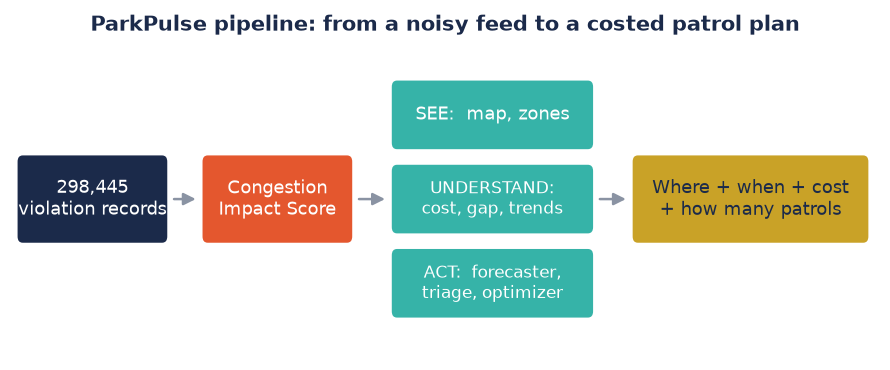
\includegraphics[width=0.95\linewidth]{fig-pipeline}
\caption{The pipeline: a noisy violation feed becomes a ranked, costed, where-and-when patrol plan.}
\end{figure}

% ---------------------------------------------------------------- how it works
\section{How it works}

\subsection{Data foundation}
Timestamps converted UTC to IST (without this, rush-hour analysis is 5.5 hours wrong). Violation types mapped to obstruction weights; vehicle types to PCU (passenger-car-unit) footprints. Built on \texttt{approved} records, with a sensitivity check on the full set, and aggregated to H3 res-9 cells ($\sim$150\,m): 2{,}534 hotspot cells.

\subsection{Congestion Impact Score (0--100)}
A geometric mean of four percentile-ranked axes, so a cell must be bad on several dimensions to rank high:
\[ \text{score} = 100 \times (\text{volume}\times\text{intensity}\times\text{exposure}\times\text{persistence})^{1/4} \]
\textbf{Volume} (with an empirical-Bayes shrink so single-event flukes do not top the list), \textbf{intensity} (how obstructive the typical violation is), \textbf{exposure} (how busy the road normally is, from an \emph{exogenous} hour-of-day utilization curve, not the recorded hour, which is how we inject ``traffic flow'' without a feed and dodge the confound), and \textbf{persistence} (how chronic). The score is built to \emph{disagree} with a raw count: their rank correlation is 0.56. Concentration is extreme (Gini 0.84): the top 1\% of cells carry 35\% of impact; 58 cells carry half.

\begin{figure}[htbp]\centering
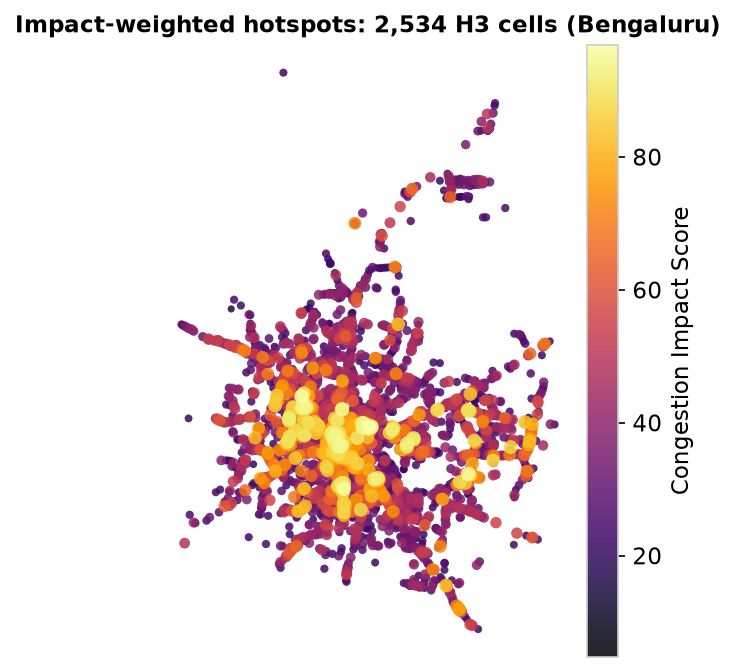
\includegraphics[width=0.56\linewidth]{fig-map}
\caption{Every H3 cell colored by Congestion Impact Score. The bright commercial core (Shivajinagar, Majestic, City Market, Malleshwaram) stands out against the cooler periphery.}
\end{figure}

\begin{figure}[htbp]\centering
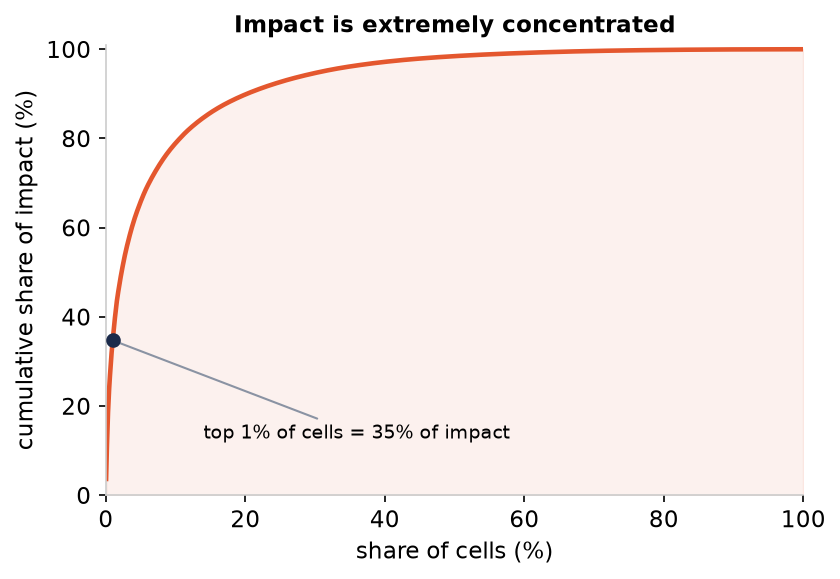
\includegraphics[width=0.62\linewidth]{fig-concentration}
\caption{Impact is extremely concentrated, so ranking by impact beats blanket coverage.}
\end{figure}

\subsection{The enforcement gap}
Recorded violations double as a map of effort. Weighting each by its impact unit (obstruction $\times$ PCU $\times$ utilization) exposes the misallocation:

\begin{table}[h]\centering\small
\begin{tabular}{lrr}
\toprule
\textbf{Time window} & \textbf{Share of effort} & \textbf{Share of impact} \\
\midrule
Pre-dawn sweep (4--5am) & 15.3\% & 4.0\% \\
Night (12--5am) & 33.7\% & 7.9\% \\
Peak-exposure hours & 28.8\% & 50.1\% \\
\bottomrule
\end{tabular}
\end{table}

A third of logged effort lands when roads are empty. ParkPulse redirects it to the peak-hour chokepoints.

\begin{figure}[htbp]\centering
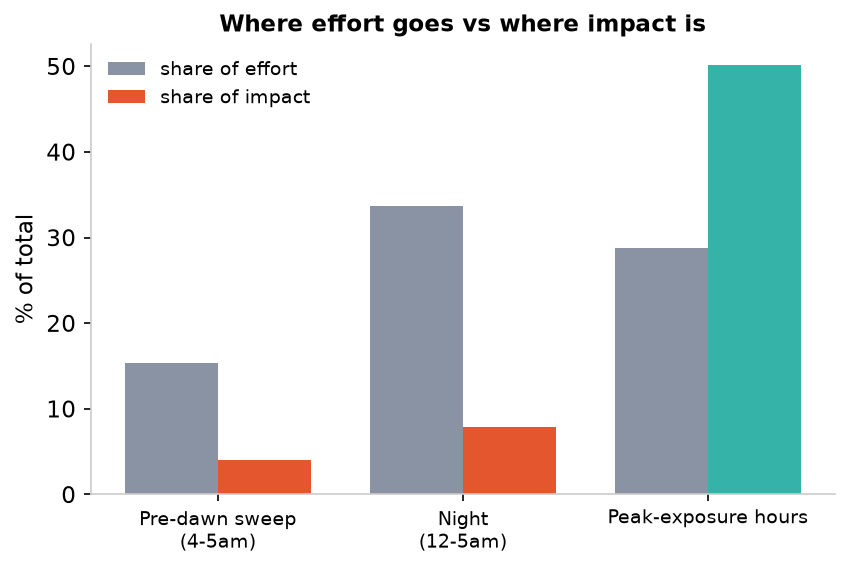
\includegraphics[width=0.66\linewidth]{fig-gap}
\caption{Where enforcement effort goes (grey) versus where congestion impact is. The night windows absorb effort while roads are empty; the peak hours are under-served.}
\end{figure}

\subsection{Ranked zones, cost, and emerging hotspots}
\textbf{Ranked zones:} the top 30 cells, each with a dominant violation, the streets involved, and an exposure-weighted window. Validated by face validity (20 of the top 20 are known chokepoints) and month-to-month stability ($\rho \approx 0.75$--$0.86$).
\textbf{Cost:} calibrating the physical delay-potential into vehicle-hours and rupees gives $\sim$574 vehicle-hours/day, $\sim$Rs 5.2 crore/year (base, with a band), the worst 20 cells carrying 31\% of it.
\textbf{Emerging hotspots:} trending each cell's \emph{share} of citywide volume over the four full months (which detrends the citywide enforcement ramp) flags 227 rising cells, 103 of them both high-impact and rising.

\subsection{Two machine-learning models}
\textbf{Forecaster (real ground truth):} predicts next-day intensity per cell on a strict temporal holdout (train Nov--Feb, test Mar--Apr). A bake-off across the gradient-boosting family picks LightGBM (Tweedie); it beats the seasonal-naive baseline by 36\% on coverage@20 (0.257 to 0.348) and dominates on calibration (Tweedie deviance 3.45 vs 90), capturing 72\% of the oracle ceiling. We tested 29 extra features and tuning; none beat the base set. Honest read: the ceiling is the data, not the model.
\textbf{False-detection triage:} about a third of reviewed reports are rejected; a separate classifier predicts which, with ROC-AUC 0.758 / PR-AUC 0.632. Flag the top 20\% most-suspect and you catch 43\% of all rejections at 64\% precision.

\begin{figure}[htbp]\centering
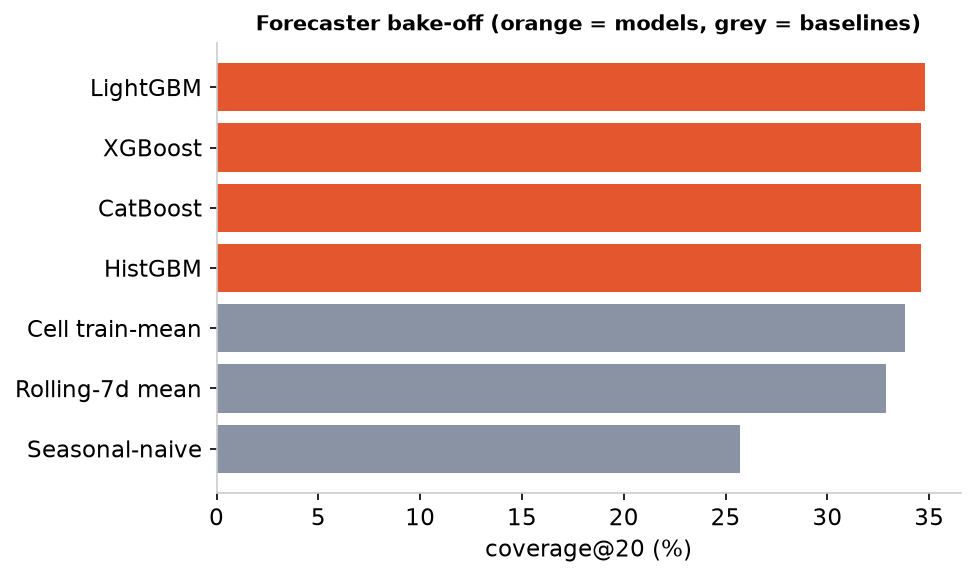
\includegraphics[width=0.66\linewidth]{fig-forecast}
\caption{Forecaster bake-off on the temporal holdout: the gradient-boosting models (orange) clear the naive baselines (grey).}
\end{figure}

\subsection{Patrol optimizer and ROI}
A greedy max-coverage optimizer assigns N beats (cell plus H3 ring) to maximize impact covered. Because the worst cells cluster, 20 beats cover 53\% of citywide impact vs 47\% for a naive top-N pick, relieving roughly Rs 77k/day of delay.

\begin{figure}[htbp]\centering
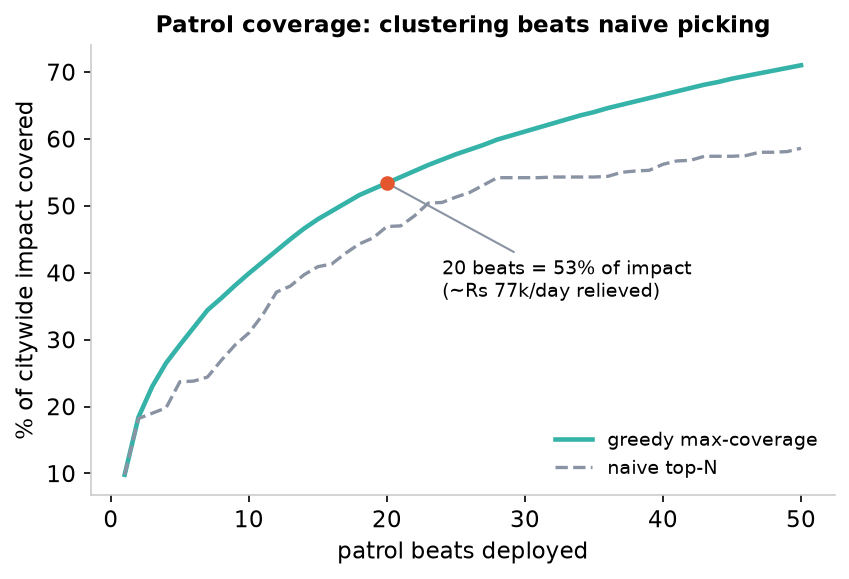
\includegraphics[width=0.66\linewidth]{fig-coverage}
\caption{Patrol coverage versus fleet size. Greedy max-coverage beats a naive top-N pick; 20 beats cover 53\% of impact.}
\end{figure}

% ---------------------------------------------------------------- results
\subsection{Is the score robust?}
A fair question is whether the ranking is an artefact of the equal weighting. It is not. Across 2{,}000 random re-weightings of the four axes (each varied up to 3x in relative importance), the ranking holds at a median Spearman of 0.97 against the shipped score, and the top-20 zones retain 18 of 20 on average. Switching from a geometric to an arithmetic mean still correlates at 0.86, and no single axis dominates: dropping any one keeps Spearman above 0.82. The ranking reflects the data's structure, not a hand-tuned weighting.

\begin{figure}[htbp]\centering
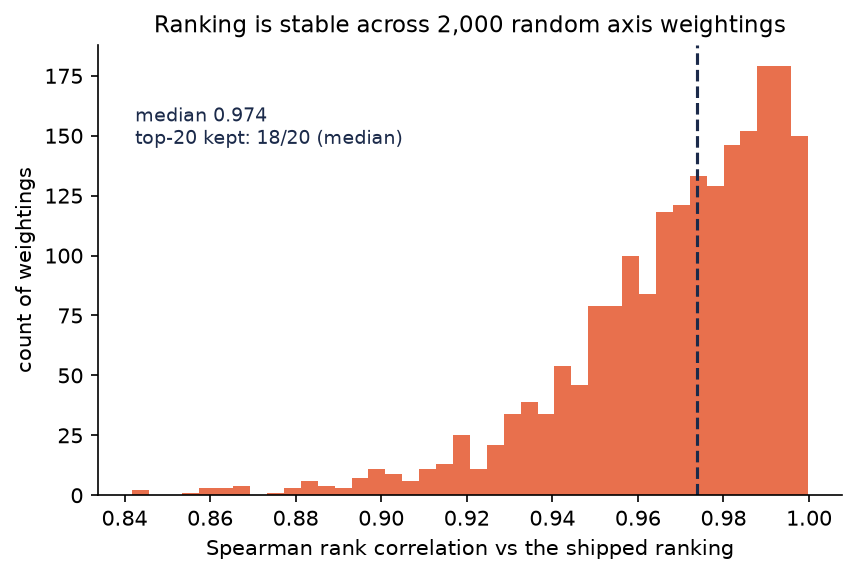
\includegraphics[width=0.62\linewidth]{fig-robustness}
\caption{Across 2,000 random axis weightings, the ranking stays close to the shipped one (median Spearman 0.97).}
\end{figure}

\section{Results at a glance}
\begin{table}[h]\centering\small
\begin{tabular}{ll}
\toprule
\textbf{What} & \textbf{Result} \\
\midrule
Hotspot cells scored & 2{,}534 (H3 res-9) \\
Impact vs raw count & rank corr 0.56 (deliberately decoupled) \\
Concentration & top 1\% of cells = 35\% of impact; 58 cells = 50\% \\
Enforcement gap & night = 34\% of effort, 8\% of impact \\
Estimated delay cost & $\sim$574 veh-hr/day, $\sim$Rs 5.2 cr/yr (band) \\
Emerging & 227 rising; 103 high-impact and rising \\
Forecaster & +36\% cov@20 vs seasonal-naive; 72\% of oracle \\
False-report triage & ROC-AUC 0.758; top-20\% flag catches 43\% \\
Patrol optimizer & 20 beats = 53\% impact, $\sim$Rs 77k/day relieved \\
Validation & face validity 20/20; stability $\rho$ 0.75--0.86 \\
\bottomrule
\end{tabular}
\end{table}

% ---------------------------------------------------------------- honesty
\section{Honesty and limitations}
\begin{itemize}[label=\textbullet]
  \item \textbf{No ground truth for impact.} The score is an engineered index, not a measurement; we validate by face validity, stability, and a robustness check. We also ship an independent OpenStreetMap cross-check (\texttt{osm\_validate.py}): the score, built without the road network, is compared against real road criticality and nearby congestion-generators, the closest thing to ground truth without a speed feed.
  \item \textbf{The enforcement confound.} We weight by exogenous exposure, never the recorded hour, and state that the forecaster predicts recorded detections under current enforcement, not pure demand.
  \item \textbf{The data can't see the evening.} Evening violations are near-absent because enforcement rarely works evenings, so we do not build an hour-by-hour schedule from the recorded hour.
  \item \textbf{Fusion-ready.} The moment a live speed feed, real road network, events calendar, or patrol roster exists, those factors become inputs and measured slowdown becomes the label. The data gap is a roadmap.
\end{itemize}

% ---------------------------------------------------------------- tech
\section{Architecture and tech}
\textbf{Pipeline:} Python (pandas, numpy, h3 v4, scikit-learn, lightgbm); each step reads committed artifacts and writes to \texttt{data/} or \texttt{outputs/}.
\textbf{Web app:} Next.js (static export) + deck.gl (\texttt{H3HexagonLayer}) + Recharts + Tailwind. Fully static, reading precomputed JSON, so it runs on a CDN with no backend and no API keys and cannot fall over under load.
\textbf{Optional enrichment:} \texttt{enrich\_osm.py} adds real road class and nearby congestion-generators from OpenStreetMap; everything downstream is graceful if it is absent.

% ---------------------------------------------------------------- roadmap
\section{Impact and roadmap}
Today, ParkPulse gives enforcement the prioritization they are missing: a ranked, costed, where-and-when plan, plus the ROI of acting on it. With one more data feed it becomes a measured, learning system: plug in live speeds for a true impact label, the OSM road graph for flow-criticality, and patrol rosters to de-bias the confound.

\end{document}
